\renewcommand{\inputfile}{\version\ - edited 2008-08-29 symODEs}
% section: Symmetries of dynamical systems
% $Author$ $Date$



\subsection{Definition of symmetry}

We consider a system of \ode's of the form
\beq
	\dot{x} = \vf(x,\lambda)
	\label{eq:difeq}
\eeq
where $\vf: \Rls{n}\times\Rls{r} \rightarrow \Rls{n}$ a $C^\infty$ mapping. When
not important we will suppress the $r$-dimensional vector of parameters
$\lambda$ in the notation.

Any compact Lie group acting on $\Rls{n}$ can be identified
with a subgroup of $\On{n}$, \cf\ for example \refref{golubII}
for a sketch of the proof. Therefore, without loss of generality
we will concentrate on subgroups $\Gamma\subseteq\On{n}$ in the following.

\begin{definition}
\label{def:symmetry}
\index{symmetry}
We call a group element $\gamma\in\On{n}$ a symmetry of \refeq{eq:difeq} if for every solution
$x(t)$, $\gamma x(t)$ is also a solution.
\end{definition}\ES{Refer to point vs contact symmetries?}

The question now arises on how to check for symmetries of \refeq{eq:difeq} since
we generally do not have knowledge of the set of solutions\ES{Rather naively put.}. Let $x(t)$ be a solution
of \ref{eq:difeq}. Then by \refDef{def:symmetry} $y(t)=\gamma x(t)$ is another solution
and therefore satisfies \refneq{eq:difeq}:
\[
 \dot{y}(t)=\vf{\PCedit{(y(t))}}=\vf(\gamma x(t))\,.
\]
On the other hand
\[
 \dot{y}(t)=\gamma \dot{x} = \gamma \vf(x(t))\,,
\]
for any solution $x(t)$. Since solutions exist for any $x\in\Rls{n}$ we are led to the following
condition for $\gamma$ to be a symmetry of \refeq{eq:difeq}:
\beq
	\vf(\gamma x) =\gamma \vf(x)
	\label{eq:equiv}
\eeq
for all $x\in\Rls{n}$. We say that $\vf$ \emph{commutes} with $\gamma$ or that $\vf$ is $\gamma$-\emph{equivariant}.
When $\vf$ commutes with all $\gamma\in\Gamma$ we say that $\vf$ is $\Gamma$-equivariant\index{equivariant}.
% When $f$ is $\gamma$-equivariant
% the \ode~ \ref{eq:difeq} remains invariant under the action of $\gamma$. 
Clearly the finite time flow $\flow{t}{\gamma x_o}$ through $\gamma x_o$
satisfies the equivariance condition $\flow{t}{\gamma x_o}=\gamma \flow{t}{x_o}$ from
definition of symmetry and uniqueness of solutions.


\index{Lorenz flow!symmetry}
For example, the vector field in Lorenz equations  \refneq{eq:lorenz} is equivariant under the group
$\Ztwo\cong\Dn{1}$ acting on \Rls{3}\ by
\[
	\Rot{\pi}(x,y,z) = (-x,-y,z)\,.
\]
Note that this transformation can be considered either as rotation by $\pi$ around the $z$ axis (hence the
group \Ztwo) or as reflection about the origin in a plane perpendicular to the $z$-axis (hence the group \Dn{1}.)

\index{Complex Lorenz flow!symmetry}
As another example, the vector field in \CLe\ \refneq{eq:CLe} is equivariant under the group \SOn{2} acting on $\Rls{5}\cong \Clx{2}\times \Rls{}$
by
\beq
 \Rot{\theta} (x,y,z) = (e^{i\theta} x, e^{i\theta} y, z)\,,\ \ \  \theta\in[0,2\pi)\,.
 \label{eq:RotCLe}
\eeq

\index{Armbruster-Guckenheimer-Holmes flow!symmetry}Finally, the symmetry group of the \AGHe~\refneq{eq:AGH} is \On{2} acting by
\begin{eqnarray*}
  \Rot{\theta}(z_1,z_2) &=& (e^{i\theta} z_1, e^{i 2\theta} z_2)\,,\ \ \  \theta\in[0,2\pi)\,,\\
  \Refl(z_1,z_2) &=& (\conj{z}_1,\conj{z}_2)\,.
\end{eqnarray*}


\subsection{Phase space stratification}

In order to understand the implications of equivariance for the solutions
of \refeq{eq:difeq} we first have to examine the way a compact
Lie group acts on \Rls{n}.

\index{group orbit} The \emph{group orbit} of $x\in\Rls{n}$ is the set
\beq
	\Gamma x = \{\gamma x: \gamma\in\Gamma\}\,.
\eeq

\begin{definition}
\label{def:stab}
\index{isotropy subgroup}\index{stabilizer}
The isotropy subgroup or stabilizer of $x\in\Rls{n}$ as
\beq
	\stab{x}=\{\gamma\in\Gamma:\gamma x=x\}\,.
\eeq
\end{definition}
Thus the isotropy subgroup describes the symmetries of a point $x$. Note that by
\refDef{def:stab} the isotropy subgroup is the largest subgroup (in the
sense of set inclusion, \cf \refeq{eq:Gorder}) that leaves $x$ fixed.
% PC commented this out: The following lemma
% relates the isotropy subgroups of points on the same group orbit.

\begin{lemma}
\label{lem:stabGorbit}
Points on the same group orbit of $\Gamma$ have conjugate isotropy subgroups:
\beq
	\stab{\gamma x}=\gamma \stab{x} \gamma^{-1}\,.
\eeq
\end{lemma}
(See \refref{golubII} for the proof.)
%
% \refLem{lem:stabGorbit} implies that
Thus we can characterize a group orbit by its \emph{type}, defined
as the conjugacy class of its isotropy subgroups.

\begin{proposition}
 Let $\Gamma$ be a compact Lie group acting on \Rls{n}. Then
 \begin{enumerate}
  \item If $\Gamma$ is finite then $|\Gamma|=|\stab{x}||\Gamma x|$.
  \item If $\Gamma$ is continuous then $\dim \Gamma = \dim \stab{x}+\dim \Gamma x$.
 \end{enumerate}
\end{proposition}
The proof can be found in \refref{golubII}. We note that
% PC commented out: a useful relation from the proof:
$\dim\Gamma x =\dim(\Gamma/\stab{x})$, where the \emph{coset space} of
a subgroup $\Sigma$  of $\Gamma$ is defined as
$\Gamma/\Sigma=\{\gamma\Sigma|\gamma\in\Gamma\}$.
Also recall that the (left) \emph{cosets} of $\Sigma$ in $\Gamma$ are the sets
$\gamma\Sigma=\{\gamma\sigma|\sigma\in\Sigma\}$.

\index{stratum}
Therefore, when $\Gamma$ is continuous each group orbit is a smooth compact manifold of dimension
$\dim \Gamma x=\dim \Gamma-\dim \stab{x}$. The union of orbits of the same type is called a \emph{stratum}
and is itself a smooth manifold. Thus \Rls{n} is stratified by the action of $\Gamma$ into
a disjoint union of strata $\Str{i}$ which are in an $1-1$ correspondence to the group orbit types(\cf~\refref{ChossLaut00} for proof.) 
Note that in general the strata do not have the same dimension. There exists a unique stratum \Str{0} of maximal
dimension that is called \emph{principal stratum}\cite{gatermannHab}. The principal stratum is open, dense 
and if $\Gamma$ is connected then \Str{0} is also connected\cite{ChossLaut00}.

\begin{definition}
 \label{def:fixedsp}
 \index{fixed-point subspace} Let $\Sigma$ be a subgroup of $\Gamma$ acting on \Rls{n}. The \fixedsp\ of $\Sigma$,
 denoted by $Fix(\Sigma)$, is the subspace of \Rls{n} containing all fixed points of $\Sigma$:
\[
	Fix(\Sigma)=\{x\in\Rls{n}\ |\ \sigma x = x\,,\ \forall \sigma\in\Sigma\}\,.
\]
\end{definition}

\Fixedsp s are invariant under equivariant dynamics. The following theorem applies:

\begin{theorem}
 Let $f:\Rls{n}\rightarrow\Rls{n}$ be $\Gamma$-equivariant and let $\Sigma$ be a subgroup of $\Gamma$. Then
\[
 f\left(Fix(\Sigma)\right)\subseteq Fix(\Sigma)\,.
\]
\end{theorem}\ES{write the proof}

This leads to:
\begin{proposition}
 Let $x(t)$ be a solution trajectory of an equivariant ODE. Then $\Sigma_{x(t)}=\Sigma_{x(0)}$ for all $t$.
\label{pro:gfInv}
\end{proposition}\ES{write the proof}

We can define a partial ordering $\preceq$ on conjugacy classes of subgroups of $\Gamma$. Let $H=\{H_i\}$ and $K=\{K_j\}$
be two such conjugacy classes. Then
\beq
	H\preceq K \Leftrightarrow H_i\subseteq K_j
	\label{eq:Gorder}
\eeq
for some representatives $H_i,\,K_j$. We refer to the partially ordered set that results from this ordering as the \emph{subgroup lattice}.

\begin{definition}
 The isotropy lattice of $\Gamma$ is the set of all conjugacy classes of isotropy subgroups
 partially ordered by $\preceq$.
\end{definition}
    \ES{
I copy Golubitsky and Stewart's definition of isotropy lattice and partial ordering (but not of subgroup lattice)
here because I am somewhat confused. Are the conjugacy classes of subgroups distinct
from the classes defined by conjugate elements of the group?
For instance in the example of \Dn{3} below, $\Ztwo(\Refl)$, $\Ztwo(\Refl \Drot)$
and $\Ztwo(\Refl \Drot^2)$ are conjugate subgroups. My interpretation is that we call this
a conjugacy class of isotropy subgroups.
On the other hand, \Dn{3} is partitioned in three classes: $\{e\},\{\Refl,\Refl\Drot,\Refl\Drot^2\}$
and $\{\Drot,\Drot^2\}$ which of course are not subgroups, except for $\{e\}$.
    }

\begin{example} % Subgroups of \Dn{3}
As an example we will consider \Dn{3}, the symmetry group of the equilateral triangle
\reffig{fig:D3triangle}, acting on $\Rls{2}\cong\Clx{}$ by
\begin{eqnarray*}
  \Drot z &=& e^{i\frac{2\pi}{3}} z\,,\\
  \Refl z  &=& \conj{z}\,.
	\label{eq:D3onR2}
\end{eqnarray*}

%%%%%%%%%%%%%%%%%%%%%%%%%%%%%%%%%%%%%%%%%%%%%%%%%%%%%%%%%%%%%%%%
\begin{figure}
    % \vspace*{-5pt}
\begin{center}
		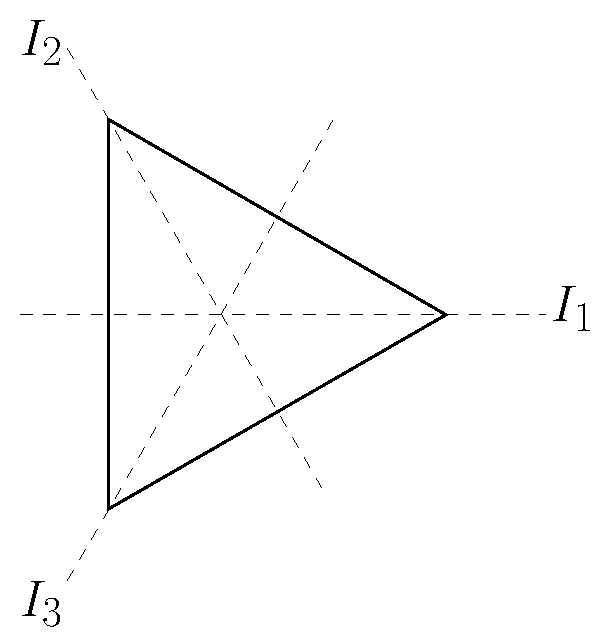
\includegraphics[width=0.25\textwidth]{../figs/D3triangle}
\end{center}
\caption[D3 symmetry illustration.]{
    {\small
    \Dn{3} leaves the equilateral triangle setwise fixed. The reflection symmetry axes have been denoted $I_i$.}}
\label{fig:D3triangle}
    \vspace*{-5pt}
\end{figure}
%%%%%%%%%%%%%%%%%%%%%%%%%%%%%%%%%%%%%%%%%%%%%%%%%%%%%%%%%%%%%%%%%

There are, up to conjugacy, three subgroups: $\Idg=\{e\}$, $\Ztwo(\Refl)$,
which is isomorphic to the subgroups generated
by $\Refl\Drot$ and by $\Refl\Drot^2$, and $\Zn{3}=\{e,\Drot,\Drot^2\}$.
The subgroup lattice is shown in \reffigpart{fig:D3lattice}{a}.
There are three classes, each corresponding to
a distinct geometrical operation: $\{e\},\{\Refl,\Refl\Drot,\Refl\Drot^2\}$
and $\{\Drot,\Drot^2\}$.


\end{example}


\begin{example}  % Isotropy subgroups of \Dn{3}

We now examine how the vertex $A$ of the triangle transforms
under the axion of \Dn{3}. Under $\Drot$ and $\Drot^2$ it is
mapped to the vertices $B$ and $C$, respectively.
Thus all vertices belong to the same group orbit and have
conjugate isotropy subgroups, from \refLem{lem:stabGorbit}.
Under $\Refl$ vertex $A$ remains fixed. Thus the isotropy
subgroup of point $A$ is $\stab{A}=\Ztwo(\Refl)$. By
\refLem{lem:stabGorbit} we have $\stab{B}=\Drot\,
\Ztwo(\Refl)\, \Drot^{-1} = \Ztwo(\Refl\Drot)$
and
    \PCedit{
$\stab{C}=\Drot^{-1}\, \Ztwo(\Refl)\, \Drot =
\Ztwo(\Refl\Drot^2)$.
    }
Next, note that $\Ztwo(\Refl)$ fixes
any point on the symmetry axis $I_1$, while $\Drot$ and
$\Drot^2$ map it to $I_2$ and $I_3$, respectively. The origin
is the only point fixed by any group operation, \ie~has
isotropy subgroup $\Dn{3}$. Finally, any point that is not on
one of the symmetry axes $I_1,\ I_2,\ I_3$ has trivial isotropy
subgroup. Thus we arrive to the following conclusions:

The isotropy subgroups are: $\stab{\{0\}}=\Dn{3}$,
$\stab{I_1^*}=\Ztwo(\Refl)\simeq\stab{I_2^*}\simeq\stab{I_3^*}$,
$\stab{\Rls{2}\backslash\{\cup I_i\}}=\Idg$, where $I_i^*$ is
used as a shortcut for $I_i\backslash\{0\}$. The fixed point
subspaces of \Dn{3}, $\Ztwo(\Refl)$, $\Ztwo(\Refl\Drot)$ and
$\Ztwo(\Refl\Drot^2)$ are the origin, $I_1$, $I_2$ and $I_3$,
respectively. The fixed point subspace of \Zn{3} is the origin
but, since \Zn{3} is a proper subgroup of \Dn{3}, it
does not qualify as isotropy subgroup of the origin
(\cf~\refDef{def:stab}.) Thus \Zn{3} is not in the isotropy
lattice of \Dn{3} acting on \Rls{2},
\cf~\reffigpart{fig:D3lattice}{b}.
    \PC{something is screwy with the \pCf\ analysis - there
        we keep \Zn{3}, I think...}

%%%%%%%%%%%%%%%%%%%%%%%%%%%%%%%%%%%%%%%%%%%%%%%%%%%%%%%%%%%%%%%%
\begin{figure}
    % \vspace*{-5pt}
\begin{center}
  (\textit{a})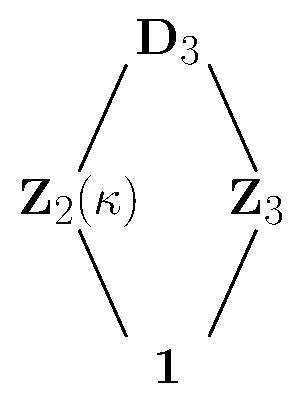
\includegraphics[width=0.105\textwidth]{../figs/D3lattice}
~~~~(\textit{b})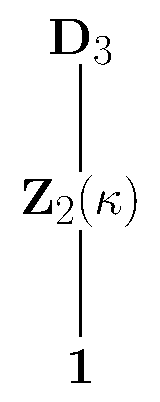
\includegraphics[width=0.05\textwidth]{../figs/D3stablattice}
\end{center}
\caption[D3 lattices]{
    {\small
    (a) \Dn{3} subgroup lattice, (b) \Dn{3} isotropy lattice}}
\label{fig:D3lattice}
    \vspace*{-5pt}
\end{figure}
%%%%%%%%%%%%%%%%%%%%%%%%%%%%%%%%%%%%%%%%%%%%%%%%%%%%%%%%%%%%%%%%%

There are three strata in correspondence with the orbit types (and with isotropy subgroups): the origin (type \Dn{3}),
$\{\cup I_i^*\}$ (type $\Ztwo(\Refl)$), and the principal stratum $\Rls{2}\backslash\{\cup I_i\}$ (type $\Idg$).

If we now consider a two dimensional system of \ode s equivariant under the action \refneq{eq:D3onR2} of \Dn{3} we
can conclude immediately that the \fixedsp s are flow invariant by \refPro{pro:gfInv}. Thus the origin has to be
a \fixedpnt\ of the flow. Moreover the principal stratum $\Rls{2}\backslash\{\cup I_i\}$ is partitioned by the symmetry
axes $I_i$ that are flow invariant into six disjoined pieces on the same group orbit of \Dn{3}.

\end{example}

A general procedure exists\cite{gatermannHab} to determine which subgroups in the subgroup lattice of a group $\Gamma$ are isotropy
subgroups when $\Gamma$ acts faithfully on $\Rls{n}$.
For each subgroup $K$ (or more precisely for each subgroup class represented by $K$)
determine the dimension of the \fixedsp. Then we trace the subgroup lattice: For each subgroup
$K$ we compare $dim(Fix(K))$ to $dim(Fix(H))$ for every $H\subseteq\Gamma$ for which $K\subset H$.
If  $dim(Fix(K))=dim(Fix(H))$ then $K$ is not an isotropy subgroup. The determination of the dimension of the
\fixedsp\ of a subgroup $K$ can be done by means of the following trace formula if an explicit representation
$\rho(K)$ of $K$ is known\ES{Or if one is able to determine the character of the representation by other means.}:
\beq
	dim(Fix(K))=\frac{1}{|K|}\sum_{\kappa\in K} \trace(\rho(\kappa))\,.
\eeq

% In general, once the subgroup lattice has been determined one goes up the lattice comparing the dimensions of fixed point subspace for


% We observe that points on reflection symmetry axis $I_1$ are in the \fixedsp\ of


% The notion of equivariance is related to the symmetries of the \ode\ \refeq{eq:difeq}. We will also
% be interested on the symmetries of solutions.

\subsection{Principal Fibre Bundles}

Assume a Lie group $\Gamma$ acts\ES{Any restriction on how it acts? In definition in Isham the term G-space is used, which I don't understand since he doesn't define it.} on a topological space $\tSp$. We call the bundle $(\tSp,\prj,\bSp)$ a \emph{$\Gamma$-bundle} if it is isomorphic to $(\tSp,\rho,\tSp/\Gamma)$. The fibres over the points of the base space $\bSp$ are the group orbits of points in $\tSp$. Thus in general \ES{Can we 
substitute ``in general'' with ``if $\Gamma$ does not act freely on $E$ then''} the bundle $E$ is not a fibre bundle since the fibres are not homeomorphic to each other. If $\Gamma$ acts freely on
$\tSp$ then the $\Gamma$-bundle is a fibre bundle with fibre $\Gamma$ and is called a \emph{principal $\Gamma$-bundle}, while $\Gamma$ is called the structure group of the bundle.

\subsection{Symmetries of solutions}

In the preceding section we concentrated on symmetries of the space on which the group acts.
We now proceed to examine the symmetries of solutions of equivariant dynamical systems.


\subsection{Moving frames}

In this section we present the method of moving coframes
    \PC{do they really say ``moving coframes'' rather than ``comoving frames''? {\bf ES}: Yes, they really do. They refer to
Cartan's method as method of ``moving frames'' and they claim it to be a special (less rigorous) case of the moving coframe method.
I don't know Cartan's method and the two papers of Fels and Olver\rf{FelsOlver98,FelsOlver99} are lengthy and technical. Olver's
book is readable but I it doesn't describe Cartan's method. I think they say ``moving'' rather than ``comoving" frames
because one only comoves in the direction of group action.}
of Fels and Olver\rf{FelsOlver98,FelsOlver99}, also \cf~\refref{OlverInv} for
a pedagogical exposition. The method can be used to generate functionally independent\ES{rechecked they are in general functionally independent.} fundamental invariants for the action
of a group $\Gamma$ on a manifold $\Manif$ under certain conditions. 
It draws from the method of moving frames of Cartan.
    \ES{cite Cartan}
Here we follow \refref{OlverInv} but first motivate the general method through an example.

Consider $\Sigma=\SOn{2}$ acting on $\Rls{5}$ by
\beq
	x \mapsto  \Rot{\theta}x\,,
	\label{eq:SO2act}
\eeq
where
\beq
	\Rot{\theta}=	\left(\barr{ccccc}
				\cos(\theta) & -\sin(\theta) & 0	   & 0		    & 0\\
				\sin(\theta) & \cos(\theta)  & 0	   & 0		    & 0\\		
				0	     & 	0	     & \cos(\theta) & -\sin(\theta) & 0\\
				0	     &  0	     & \sin(\theta) & \cos(\theta) & 0\\
				0	     &  0	     & 0	    & 0		   & 1\\	
			\earr\right)\,,\ \ \theta\in[0,2\pi)\,.
\eeq
Note that this is the same action as in \refeq{eq:RotCLe} but now we do not make the identification
	$\Rls{5}\cong \Clx{2}\times \Rls{}$. As we will see in \refchap{chap:lasers} the following have direct application in symmetry reduction
of \CLe. Choose coordinates $x_1,x_2,y_1,y_2,z$ on $\Rls{5}$, related to the complex coordinates
of \refeq{eq:RotCLe} by $x=x_1+i x_2$, $y=y_1+i y_2$. Note that the \fixedsp\
of the action of $\SOn{2}$ defined above is the $z$-axis.
%     \PC{where is \fixedsp\ defined? {\bf ES}: Sorry, it's there now. See \refDef{def:fixedsp}}.
The isotropy subgroup of the $z$-axis is thus
$\SOn{2}$, while the isotropy subgroup of $\Manif^*\equiv\Rls{5}\backslash\{x_1=x_2=y_1=y_2=0\}$ is the identity element.

\begin{definition}
\label{def:free}
\index{free}
A group $\Gamma$ acts freely on $\Manif$ if all isotropy subgroups are trivial: \stab{x}=\{e\} for all $x\in \Manif$.
$\Gamma$ acts locally freely if all isotropy subgroups are discrete subgroups of $\Gamma$.
\end{definition}

Thus $\Sigma$ does not act freely on $\Rls{5}$ but acts freely on $\Manif^*$. If we don't
restrict $\theta$ in $[0,2\pi)$ then the group $\Rg{}$ acts locally freely on $\Manif^*$
since the isotropy subgroup is the discrete subgroup $2\pi\mathbb{Z}$ of integer multiples of $2\pi$.

Here we will need to generalize\ES{This definition might belong to the section on phase space stratification.} 
the notion of isotropy subgroups by introducing the isotropy subgroup of a set and also introduce the
global isotropy subgroup.

\begin{definition}
\label{def:StabS}
\index{isotropy subgroup}
 The isotropy subgroup of a subset $S\subset \Manif$ is the set
 \[
  	\stab{S}=\{\gamma\in\Gamma:\gamma S=S\}\,.
 \]
\end{definition}

\begin{definition}
\label{def:GlobStab}
\index{isotropy subgroup!global}
 The global isotropy subgroup of a subset $S\subset \Manif$ is the set
 \[
  	\globstab{S}=\bigcap_{x\in S} \stab{x} = \{\gamma\in\Gamma:\gamma x=x\,,\ \forall x\in S\}\,.
 \]
\end{definition}

\begin{definition}
\label{def:faithfull}
\index{faithful}
A group $\Gamma$ acts faithfully (or effectively) on $\Manif$ if it has trivial global isotropy subgroup.
\end{definition}

\begin{definition}
\label{def:regular}
\index{regular}\index{semi-regular}
A group $\Gamma$ acts semi-regularly on $\Manif$ if all its orbits have the same dimension. If in addition for each point $x\in \Manif$
there exists an arbitrarily small neighborhood $U$ such that each orbit of $\Gamma$ intersects $U$ in a pathwise connected subset, then the group
acts regularly.
\end{definition}
\ES{Think of regular versus semi-regular action as the group orbits being circles versus filling a 2-torus. I'll try to find a specific example of semiregular action.}

Thus $\Sigma=\SOn{2}$ acts regularly on $\Manif^*$ but not on $\Rls{5}$. For groups acting regularly we can define a cross-section for the group orbits.

\begin{definition}
\label{def:cross-section}
\index{cross-section}
Let $\Gamma$ act regularly on a $n$-dimensional manifold $\Manif$ with $r$-dimensional orbits. Define a (local) \emph{cross-section}
to be an $(n-r)$-dimensional submanifold $K$ of $\Manif$ such that $K$ intersects each orbit transversally and at most once.
\end{definition}

\begin{proposition}[\cite{OlverInv}]
 If a Lie group $\Gamma$ acts regularly on a manifold $\Manif$, then one can construct a local cross-section
 passing through any point $x\in \Manif$.
\end{proposition}

A cross-section $K$ can be defined by means of level sets of functions $K_i(x)=c_i$,
where $x\in V$ and $i=1,\ldots,r$. If the $K_i(x)$
coincide with the local coordinates $x_i$ on the manifold $V$, \ie~$K_i(x)=x_i$,
then we call $K$ a \emph{coordinate cross
section}. In our example we can define a coordinate cross-section for the action of
$\Sigma=\SOn{2}$ on $\Rls{5}\backslash\{x_1=x_2=y_1=y_2=0\}$  by, for instance, $x_1=0$.

We can now construct a moving frame for the action \refneq{eq:SO2act} of $\SOn{2}$ as follows.
We write out explicitly the
group transformations:
\beq
\begin{split}
 	\overline{x}_1 &= x_1 \cos\theta - x_2 \sin\theta\cont
	\overline{x}_2 &= x_1 \sin\theta + x_2 \cos\theta\cont
	\overline{y}_1 &= y_1 \cos\theta - y_2 \sin\theta\cont
	\overline{y}_2 &= y_1 \sin\theta + y_2 \cos\theta\cont	
	\overline{z} &= z\,.
	\label{eq:CLEexplSO2}
\end{split}
\eeq
Then make $\overline{x}_1$ equal to the constant in the choice of cross-section, \ie~set $\overline{x}_1=0$. Thus, we can solve
the first of \refeq{eq:CLEexplSO2} for the group parameter $\theta$ and substitute in the remaining equations. We get
\beq
\begin{split}
	\theta &= 2 \tan^{-1}\frac{-x_2+\sqrt{x_1^2+x_2^2}}{x_1} \cont
	\overline{x}_2 &= \sqrt{x_1^2+x_2^2} \cont
	\overline{y}_1 &= \frac{x_2 y_1-x_1 y_2}{\sqrt{x_1^2+x_2^2}}\cont
	\overline{y}_2 &=\frac{x_1 y_1+x_2 y_2}{\sqrt{x_1^2+x_2^2}}\,.
	\label{eq:invLaser}
\end{split}
\eeq
\ES{The solution $\theta = 2 \tan^{-1}\frac{-x_2+\sqrt{x_1^2+x_2^2}}{x_1}$ was returned by Mathematica. If we use
$\theta = \tan^{-1}\frac{x_2}{x_1}$ our results are multiplied by $sgn(x_2)$.} We note that $\overline{x}_2,\overline{y}_1,
\overline{y}_2,\overline{z}$ are $\SOn{2}$
invariant. In fact they are the \emph{fundamental invariants} for our problem: any other invariant can be expressed
as a function of $\overline{x}_2,\overline{y}_1, \overline{y}_2,\overline{z}$ and they are functionally independent.
Thus they serve to distinguish orbits in the neighborhood of the cross-section, \ie~two points lie on the same group
orbit if and only if all the fundamental invariants agree.

 The \emph{normalization} procedure for the computation of invariants applied in the example of $\SOn{2}$ can be applied
in much more general situations as follows. Assume $\Gamma$ acts (locally) freely\ES{The condition of free
action can be relaxed \cite{OlverInv}.} on \Manif\  and
thus $\Gamma$-orbits have the same dimension, say $r$, as $\Gamma$.  Choose a coordinate cross-section $K=\{x_1=c_1,\ldots,x_r=c_r\}$.
defined by the first $r$ coordinates (relabel coordinates as necessary.) Introduce local coordinates $g=(g_1,\ldots,g_r)$ on $\Gamma$ in
the neighborhood of the identity. Write out explicitly the group transformations:
\beq
	\overline{x}= g.x = w(g,x)\,.
	\label{eq:transNorm}
\eeq
Equating the first $r$ components of the function $w$ to the constants in the definition
of the cross-section $K_i(x)=c_i$ yields the \emph{normalization equations} for $K$:
\beq
	\overline{x}_1=w_1(g,x)=c_1,\ldots,\overline{x}_r=w_r(g,x)=c_r\,.
	\label{eq:normalization}
\eeq
From the definition of cross-section and the Implicit Function Theorem the normalization equations
\refneq{eq:normalization} can always be solved for the group parameters in terms of $x$,
yielding the \emph{moving frame} associated with $K$: $g=\gamma(x)$. Substitution
of the moving frame equation back to \refeq{eq:transNorm} will yield the $n-r$
fundamental invariants. For proof \cf~\refrefs{FelsOlver98,FelsOlver99}.

The power of the method shows in the calculation of invariants for groups acting on
a high-dimensional space. Consider for example the
task of computing invariants for the standard action of $\SOn{2}$ on $\Clx{n}\cong\Rls{2n}$ defined by
\beq
	\left(\barr{cc} \overline{b}_k \\ \overline{c}_k\earr \right)=\left(\barr{cc}
			    			\cos(k\theta) & -\sin(k\theta)\\
						\sin(k\theta) & \cos(k\theta)\\
			   			\earr\\	
						\right) \left(\barr{cc} b_k \\ c_k\earr\right)\,,\ \ k=1,\ldots n\,.
	\label{eq:SO2stand}
\eeq
with $b_k,c_k\in\Rls{}$. The Gr\"{o}bner basis methods usually perform poorly as $n$ becomes larger than six\ES{I need to quote
the literature or try it to fully justify this.}. On a 1GHz Pentium III processor the fundamental invariants for $n=16$, for the cross
section $b_1=0$, were computed in approximately 130s. Most importantly the time was mostly
spend in simplification of expressions.
If one only wants to project equivariant dynamics on the \reducedsp\ then the moving frame method,
through its geometric interpretation, can be used to perform the projection without explicit knowledge of the fundamental invariants.
This idea will become clear in the example of \reducedsp\ projection
for \CLe.\ES{refer to appropriate section when written.} The fundamental invariants for \SOn{2} acting as in \refeq{eq:SO2stand} with
$n=6$ calculated with the method of moving frames are listed in \reftab{tab:SO2n6}. Note another advantage of the method: no syzygies are present.

\begin{table}
\label{tab:SO2n6}
\[
\begin{array}{ll}
  \sqrt{b_1^2+c_1^2} & \\
 \frac{-b_1^2 b_2+b_2 c_1^2-2 b_1 c_1 c_2}{b_1^2+c_1^2} & \frac{2 b_1 b_2 c_1-b_1^2 c_2+c_1^2 c_2}{b_1^2+c_1^2} \\
 \frac{-3 b_1^2 b_3 c_1+b_3 c_1^3+b_1^3 c_3-3 b_1 c_1^2 c_3}{\left(b_1^2+c_1^2\right){}^{3/2}} & \frac{-b_1^3 b_3+3 b_1 b_3 c_1^2-3 b_1^2 c_1 c_3+c_1^3
c_3}{\left(b_1^2+c_1^2\right){}^{3/2}} \\
 \frac{b_4 \left(b_1^4-6 b_1^2 c_1^2+c_1^4\right)+4 b_1 c_1 \left(b_1^2-c_1^2\right) c_4}{\left(b_1^2+c_1^2\right){}^2} & \frac{4 b_1 b_4 c_1 \left(-b_1^2+c_1^2\right)+\left(b_1^4-6
b_1^2 c_1^2+c_1^4\right) c_4}{\left(b_1^2+c_1^2\right){}^2} \\
 \frac{b_5 c_1 \left(5 b_1^4-10 b_1^2 c_1^2+c_1^4\right)-b_1 \left(b_1^4-10 b_1^2 c_1^2+5 c_1^4\right) c_5}{\left(b_1^2+c_1^2\right){}^{5/2}} & \frac{b_1
b_5 \left(b_1^4-10 b_1^2 c_1^2+5 c_1^4\right)+c_1 \left(5 b_1^4-10 b_1^2 c_1^2+c_1^4\right) c_5}{\left(b_1^2+c_1^2\right){}^{5/2}} \\
 \frac{b_6 \left(-b_1^6+15 b_1^4 c_1^2-15 b_1^2 c_1^4+c_1^6\right)-2 b_1 c_1 \left(3 b_1^4-10 b_1^2 c_1^2+3 c_1^4\right) c_6}{\left(b_1^2+c_1^2\right){}^3}
& \frac{2 b_1 b_6 c_1 \left(3 b_1^4-10 b_1^2 c_1^2+3 c_1^4\right)+\left(-b_1^6+15 b_1^4 c_1^2-15 b_1^2 c_1^4+c_1^6\right) c_6}{\left(b_1^2+c_1^2\right){}^3}
\end{array}
\]
\caption[Fundamental invariants for SO(2), n=6.]{Fundamental invariants for the standard action of \SOn{2} on \Rls{6}}
\end{table}

